\begin{figure}[H]
\centering
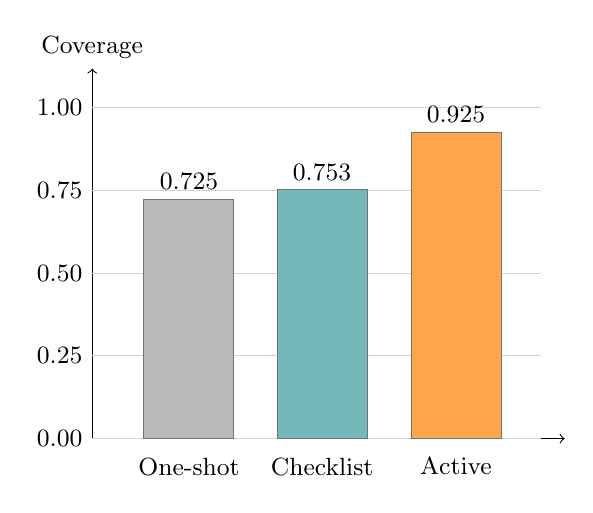
\begin{tikzpicture}[font=\small]
\draw[->] (0,0) -- (0,4.7) node[above] {Coverage};
\draw[->] (0,0) -- (6.0,0);
\draw[gray!35] (0,0.00) -- (5.7,0.00);
\node[left] at (0,0.00) {0.00};
\draw[gray!35] (0,1.05) -- (5.7,1.05);
\node[left] at (0,1.05) {0.25};
\draw[gray!35] (0,2.10) -- (5.7,2.10);
\node[left] at (0,2.10) {0.50};
\draw[gray!35] (0,3.15) -- (5.7,3.15);
\node[left] at (0,3.15) {0.75};
\draw[gray!35] (0,4.20) -- (5.7,4.20);
\node[left] at (0,4.20) {1.00};
\filldraw[fill=gray!55, draw=black!55] (0.65,0) rectangle (1.80,3.04);
\node[above] at (1.23,3.04) {0.725};
\node[below, align=center] at (1.23,-0.12) {One-shot};
\filldraw[fill=teal!55, draw=black!55] (2.35,0) rectangle (3.50,3.16);
\node[above] at (2.92,3.16) {0.753};
\node[below, align=center] at (2.92,-0.12) {Checklist};
\filldraw[fill=orange!70, draw=black!55] (4.05,0) rectangle (5.20,3.89);
\node[above] at (4.62,3.89) {0.925};
\node[below, align=center] at (4.62,-0.12) {Active};
\end{tikzpicture}
\caption{Mean reference coverage across eight synthetic workflow scenarios.}
\label{fig:overall-coverage}
\Description{Bar chart comparing mean reference coverage for one-shot, checklist, and active elicitation methods.}
\end{figure}
